\subsection{Introduction}
\begin{frame}{Shrinkage Methods}{Introduction}
    \begin{itemize}
        \item The idea is to fit a model containing all $p$ predictors using a technique \textit{regularizes} the coefficient estimates. \pause 
        $\rightarrow$ Shrinks the coefficient estimates towards zero. \pause 
        
        \item Shrinking the coefficient estimates can significantly reduce their variance. \pause 
        
        \item  The two best-known techniques for shrinking the regression coefficients towards zero are \textbf{ridge regression} and the \textbf{lasso}.

    \end{itemize}
\end{frame}

\subsection{Ridge Regression}
\begin{frame}{Shrinkage Methods}{Ridge Regression}

\begin{itemize}
    \item Recall that OLS fitting procedure estimates $\beta_0 , \beta_1 , \cdots , \beta_p$ using the values that minimize \pause
    
    \begin{equation}
        RSS = \sum_{i=1}^n (y_i - \beta_0 - \sum_{j=1}^p  \beta_j x_{ij} )^2
    \end{equation} \pause 

    \item \textit{Ridge regression} is very similar to OLS, except that the coefficients ridge are estimated by minimizing a slightly different quantity. \pause 

    \begin{equation*}
        \sum_{i=1}^n (y_i - \beta_0 - \sum_{j=1}^p  \beta_j x_{ij} )^2 + \lambda \sum_{j=1}^p \beta_j^2 = RSS + \lambda \sum_{j=1}^p \beta_j^2,
    \end{equation*} \pause 

    where $\lambda \geq 0$ is a \textit{tuning parameter} to be determined separately.
\end{itemize}
    
\end{frame}

\begin{frame}{Shrinkage Methods}{Ridge Regression}

        \begin{equation} \label{eq:ridge}
        \sum_{i=1}^n (y_i - \beta_0 - \sum_{j=1}^p  \beta_j x_{ij} )^2 + \lambda \sum_{j=1}^p \beta_j^2 = RSS + \lambda \sum_{j=1}^p \beta_j^2,
    \end{equation} \pause 

    Equation (\ref{eq:ridge}) trades off two different criteria: \pause
    
    \begin{enumerate}
        \item As with OLS, ridge regression seeks coefficient estimates that fit the data well, by making the RSS small. \pause 

        \item The term \textcolor{blue}{$ \lambda \sum_{j=1}^p \beta_j^2$} is the \textit{shirkage penalty}.  \\ \pause 
        $\rightarrow$ is small when $\beta_0 , \beta_1 , \cdots , \beta_p$ are close to zero. \pause \\ 
        $\rightarrow$ It has the effect of shrinking $\beta_j$ towards zero. \pause     
    \end{enumerate}

    $\lambda$ serves to control the impact of these two terms on the coefficient estimates. \pause 

    \begin{itemize}
        \item When $\lambda = 0$, the penalty term has no effect. The results are the OLS estimates. \pause 
        \item When $\lambda \rightarrow \infty$, the impact of the shrinkage penalty grows, and the ridge regression coefficient estimates will approach zero.
    \end{itemize}
    
\end{frame}

\begin{frame}{Shrinkage Methods}{Ridge Regression}
    \begin{itemize}
        \item OLS generates only one set of coefficient estimates. \pause 
        
        \item But ridge regression will produce a different set of coefficient estimates, $\hat{\beta}^R_\lambda$, for each value of $\lambda$. \pause 
        
        \item Selecting a good value for $\lambda$ is critical; we defer this discussion later, where we use cross-validation. \pause 

        \item The disadvantage is that ridge will include all $p$ predictors in the final model. \pause 
        
        \item The penalty $\lambda \sum \beta_j^2$ in (\ref{eq:ridge}) will shrink all of the coefficients \textbf{towards zero}, but it will not set any of them exactly to zero (unless $\lambda = \infty$). \pause 
        
        \item This may not be a problem for prediction accuracy. \pause 
        
        \item But it can create a challenge in model interpretation.
    \end{itemize}
\end{frame}


\subsection{Lasso Regression}
\begin{frame}{Shrinkage Methods}{Lasso Regression}

\begin{itemize}
    \item The lasso is an alternative that overcomes the main disadvantage of ridge regression. \pause 
    
    \item The lasso coefficients, $\hat{\beta}_\lambda^L$ , minimize the quantity \pause 

    \begin{equation} \label{eq:lasso}
        \sum_{i=1}^n (y_i - \beta_0 - \sum_{j=1}^p  \beta_j x_{ij} )^2 + \lambda \sum_{j=1}^p | \beta_j | = RSS + \lambda \sum_{j=1}^p | \beta_j |,
    \end{equation} \pause 

    \item As ridge regression, the lasso shrinks the coefficient estimates towards zero. \pause 
    
    \item However, this penalty has the effect of forcing some of the coefficient estimates to be \textbf{exactly equal to zero} when $\lambda$ is sufficiently large. \\ \pause 
    $\rightarrow$ Lasso performs variable selection. \pause 

    \item We say that the lasso yields \textit{sparse models}: models that involve only a subset of the variables. \pause

    \item Selecting a good value of $\lambda$ for the lasso is also critical. 
    
\end{itemize}
    
\end{frame}

\subsection{Another Formulation for Ridge Regression and the Lasso}
\begin{frame}{Shrinkage Methods}{Another Formulation for Ridge Regression and the Lasso}

The ridge and lasso regression coefficient estimates solve the problems: \pause

        \begin{equation}\label{eq:min-ridge}
        \underset{\beta}{\text{minimize}} \left\{     \sum_{i=1}^n \left(y_i - \beta_0 - \sum_{j=1}^p  \beta_j x_{ij} \right)^2  \right\} \text{ subject to }   \sum_{j=1}^p \beta_j^2 \leq s
    \end{equation} \pause 

    \begin{equation}\label{eq:min-lasso}
        \underset{\beta}{\text{minimize}} \left\{     \sum_{i=1}^n \left(y_i - \beta_0 - \sum_{j=1}^p  \beta_j x_{ij} \right)^2  \right\} \text{ subject to }  \sum_{j=1}^p |\beta_j| \leq s
    \end{equation} \pause \\

We find the coefficient that lead to the smallest RSS, subject to the constraint that there is a \textit{budget} $s$ forr how large the penalty can be. \pause 

    $\rightarrow$ $\forall \, \lambda \, \exists \, s$, such that the equation (\ref{eq:min-ridge}) will give the ridge estimates. \pause \\ 
    $\rightarrow$ $\forall \, \lambda \, \exists \, s$, such that the equation (\ref{eq:min-lasso}) will give the lasso estimates. 

\end{frame}

\begin{frame}{Shrinkage Methods}{Another Formulation for Ridge Regression and the Lasso}

\begin{itemize}
    \item When $p=2$, \pause 
        \begin{equation}
        \begin{aligned}
            \text{Rigde: } &\beta_1^2 + \beta_2^2 \leq s \qquad\qquad&
            \text{Lasso: } &|\beta_1 | + |\beta_2 | \leq s
        \end{aligned}    
        \end{equation} \pause 
    \item Let the OLS solution be $\hat{\beta}$. \pause 
    \item Let's represent the contours of $\hat{\beta}$ as ellipses centered around $\hat{\beta}$. \pause
    
    \begin{figure}
        \centering
        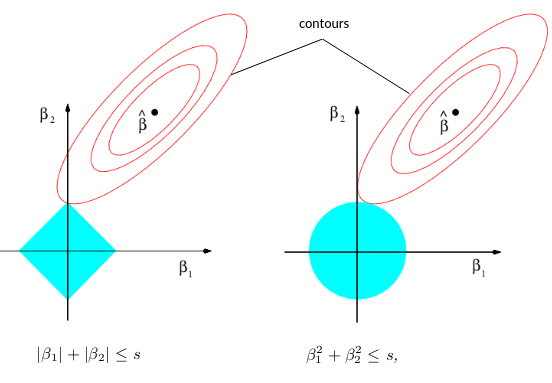
\includegraphics[height=4.5cm]{shrinkage/ridge-lasso.png}
    \end{figure} 
    
%    \item Coefficient are given by the first point at which an ellipse contacts the constraint region. 

%    \item Ridge regression has a circular constraint with no sharp points, this intersection will not generally occur on an axis, and so the ridge regression coefficient estimates will be exclusively non-zero. 

%    \item Lasso constraint has corners at each of the axes, and so the ellipse will often intersect the constraint region at an axis. When this occurs, one of the coefficients will equal zero.


\end{itemize}


\end{frame}


\subsection{Selecting the Tuning Parameter}
\begin{frame}{Shrinkage Methods}{Selecting the Tuning Parameter}
    \begin{itemize}
    \item To choose the best value of $\lambda$ we use cross-validation. \pause 
    
    \item We choose a grid of $\lambda$ values, and compute the cross-validation error for each value of $\lambda$. \pause

    \item We then select the tuning parameter value for which the cross-validation error is smallest. \pause 

    \item Finally, the model is re-fit using all of the available observations and the selected value of the tuning parameter.
\end{itemize}
\end{frame}